\section{Forced Alignment for other languages}

So far, only audio and transcripts in English were considered. A fully automated solution however should be able to align text and audio in any other language. Because of linguistic characteristics like sound patterns and morphology the results might vary a lot between languages when tested under identical circumstances. To get some intuition about the influence of language and whether above conclusions are transferable to other languages, the pipeline was evaluated on the German samples received from \textit{ReadyLingua}.

\subsection{Inferring German transcripts}

Enabling the pipeline to handle German samples means training a German \ac{ASR} as its core element. This requires minimal modifications to the network architecture, because German transcripts use a different alphabet. As mentioned before, the apostrophe is far less common in German than it is in English and was therefore dropped. On the other hand, umlauts are very common in German and were added to the 26 ASCII characters. Since the alphabet represents all possible labels, the output layer in the model needs to be changed to contain 31 units (one for each character in the alphabet, the three umlauts, space plus a blank token) instead of the 29 units used for English.

Training an \ac{ASR} model for German and plotting a learning curve also requires amounts of training data on a similar scale like the \ac{CV} corpus used for English. Since at the time of this writing, the \ac{CV} corpus was still a work in progress, datasets for languages other than English were not available. High-Quality speech corpora for \ac{ASR} are generally hard to find, especially considering the number of samples needed to train a \ac{RNN}. There are corpora for \ac{ASR} in German, but those are often liable to pay costs. An extensive list of German corpora for various purposes can be found at the \ac{BAS}\footnote{\url{https://www.phonetik.uni-muenchen.de/Bas/BasKorporaeng.html}}, including exotic corpora like the \textit{ALC} corpus\footnote{\url{http://www.bas.uni-muenchen.de/forschung/Bas/BasALCeng.html}} containing recordings of intoxicated people. Some of the corpora on this list are free for scientific usage and have been used by \cite{budget} to train their German \ac{ASR} model with transfer-learning. However, not all of these corpora are targeted at \ac{ASR} and their quality is often unknown.

\subsection{Data augmentation}

Integrating new raw data means preprocessing the audio (e.g. resampling) and the text (e.g. normalization, tokenization) to make sure it exhibits the same properties as the other corpora and the data conforms to the target format. This step is usually very time consuming, often taking most of the project time. Because no ASR corpus for German was readily available, training was done on the data received from \textit{ReadyLingua} as a start. The alignment between audio and transcript in this corpus was done manually and is therefore very accurate. Audio and text were already preprocessed in the IP8 project and the metadata was processed and stored as a corpus. The individual training samples could therefore be transformed to the format expected by the Mozilla implementation of \textit{DeepSpeech} (and thus by the simplified model) with comparably little effort. Also, the samples exhibited similar properties (average audio and transcript length) like the \ac{CV} corpus (refer to table \ref{corpora_stats}). However, the total length of the samples in the training set was only about one and a half hours, which was much less than the 1000+ minutes in the \ac{CV} corpus and certainly not enough for the $1.000$ minutes needed to plot a learning curve like to the one made for English. 

An easy way to get more training data is augmenting existing data by synthesizing new data from it. This is particularly easy for audio data, which can be distorted in order to get new samples corresponding to the same transcript. The following distortions were applied in isolation to each sample in the training set:

\begin{itemize}
	\item \textbf{Shifting}: The frames in the input signal were zero-padded with samples corresponding to a random value between $0.5$ and $1.5$ seconds, shifting the signal to the right, i.e. starting the signal later. This resulted in one additional synthesized sample for each original sample. Shifting to the left was not done to prevent cropping parts of the speech signal.
	\item \textbf{Echo}: The presence of echo can be generated with the Pysndfx library\footnote{\url{https://github.com/carlthome/python-audio-effects}} using random values for delay and damping. This resulted in one additional sample.
	\item \textbf{Pitch}: The pitch of the signal was increased or decreased. Increasing and decreasing was done using two different random factors, resulting in two additional samples. This can be seen as a rudimentary way to simulate a female from a male speaker or vice versa.
	\item \textbf{Speed}: Faster or slower speaking rates can be simulated by "stretching" or "compressing" the signal while preserving the pitch. Similar to the change in pitch, two different random factors were use to change the tempo. This resulted in two additional samples.
	\item \textbf{Volume}: The loudness of the speaker was artificially reduced or increased by a random value within the range of $[-15..-5]$ resp. $[5..15]$ db. This resulted in two additional sample.
\end{itemize}

With above methods eight synthetisized samples can be created for each original sample from the corpus. It turned out however that this was still not enough to plot a learning curve. To augment the data to the 1.000 minutes needed, additional samples were created using random combinations of the distortions. The random parameters differed from the ones used before to prevent overfitting to the distortion. Table \ref{corpus_synth_stats} shows the corpus statistics before and after data augmentation.

\begin{table}[!htbp]
	\centering
	\begin{tabular}{lrrrr}
		\toprule
		\thead{} & \thead{total audio length} & \thead{\# samples} & \thead{Ø sample length (seconds)} \\
		\midrule
		before augmentation & $1:36:09$ & $1,700$ & $2.89$ \\ 		
		after augmentation & $16:40:00$ & $18,955$ & $3.16$ \\ 		
		\bottomrule
	\end{tabular}
	\caption{Comparison of \ac{RL} corpus before and after data augmentation (training set only)}
	\label{corpus_synth_stats}
\end{table}


\subsection{Creating a Language Model for German}

Since the \ac{ASR} stage in the pipeline uses a spell-checker querying a \ac{LM} to post-process the results a $5$-gram model similar to the one created by Mozilla needed to be trained first. The following sections require understanding some methods of $n$-grams like smoothing, discount and backoff. A short explanation of how $n$-grams work is given \hyperref[n-gram-summary]{in the appendix}.

\subsection{Creating a raw text corpus}

To train a $n$-gram model for German, a raw text corpus of German Wikipedia articles was used as corpus. Like the English $n$-gram from Mozilla KenLM \parencite{kenlm} was used to estimate the probabilities. The articles were pre-processed to meet the requirements of \textit{KenLM}. It was normalized as follows 

\begin{itemize}
	\item remove Wiki markup
	\item remove punctuation
	\item make everything lowercase
	\item \textbf{Unidecoding}: translate accentuated characters (like \code{è,é,ê}, etc.) and special characters (like the German \textit{ß}) to their most similar ASCII-equivalent (\code{e} resp. \code{ss}). This process helps accounting for ambiguous spelling variants of the same word and misspelled words. It also reduces the number of unique words by reducing different versions to a normalized variant. A special case are umlauts. Although also not part of the ASCII code set, they were kept as-is because they are very common in German.
	\item \textbf{Tokenization}: Because \textit{KenLM} expects the input as sentences (one sentence per line), the raw text was further tokenized into sentences and words using NLTK \parencite{nltk}. 
	\item \textbf{Numeric tokens}: Word tokens that are purely numeric (such as year numbers) are replaced with the special token \code{<num>}. Although such tokens occur frequently in the Wikipedia articles, they are unwanted in the corpus because they represent values and do not carry any semantic meaning. Because there is a infinite number of possible numeric tokens, they were all collapsed to the same normalized token.
\end{itemize}

The corpus was saved as text file containing one normalized sentence per line. The special tokens \code{<s>} and \code{</s>} are used to mark beginnings and endings of sentences as well as the \code{<unk>} token which is traditionally used to represent \ac{OOV} words. They are however not part of the corpus because they are added automatically by \textit{KenLM}.

The following lines are an excerpt of a article in the German Wikipedia along with its representation in the corpus.

\begin{displayquote}[German Wikipedia article about Speech Recognition\footnote{\url{https://de.wikipedia.org/wiki/Spracherkennung}}]
	Die Größe des Wörterbuchs hängt stark von der Sprache ab. Zum einen haben durchschnittliche deutschsprachige Sprecher mit circa 4000 Wörtern einen deutlich größeren Wortschatz als englischsprachige mit rund 800 Wörtern. Außerdem ergeben sich durch die Flexion in der deutschen Sprache in etwa zehnmal so viele Wortformen, wie in der englischen Sprache, wo nur viermal so viele Wortformen entstehen.
\end{displayquote}

\begin{lstlisting}[numbers=left, caption=Representation in corpus]
die grösse des wörterbuchs hängt stark von der sprache ab
zum einen haben durchschnittliche deutschsprachige sprecher mit circa <num> wörtern einen deutlich grösseren wortschatz als englischsprachige mit rund <num> wörtern
ausserdem ergeben sich durch die flexion in der deutschen sprache in etwa zehnmal so viele wortformen wie in der englischen sprache wo nur viermal so viele wortformen entstehen
\end{lstlisting}

Like for the English spell checker, three vocabularies containing the $40.000$, $80.000$ and $120.000$ most frequent words from the corpus was created. The words from these vocabularies make up $87.75\%$, $90.86\%$ resp. $93.36\%$ of the total number of words in the corpus. It is expected that the optimal number of words in the vocabulary is higher for German than for English. This is due to the fact that different flexions of the same word are very common in German due to grammatical conjugations (different forms for the same verb) and declinations (different cases for the same noun). Therefore German tends to apply a wider range of words and the size of vocabulary had to be increased. Handling the different flexions would require lemmatization and/or stemming the corpus in order to reduce them to a common base form. This has not been done for simplicity and time constraints. It is also doubtful whether this would actually help improving the quality of inferred transcripts, since humans do not speak in lemmata or stems.

\subsection{Training the \ac{LM}}

The final corpus contained data from 2,221,101 Wikipedia articles (42,229,452 sentences, 712,167,726 words, 8,341,157 unique words). This corpus was used to train a $5$-gram \ac{LM} using \textit{KenLM}. \textit{KenLM} uses \textit{Kneser-Ney Smoothing} and some optimization techniques called \textit{quantization} and \textit{pointer compression}. 

\subsubsection{Data structures}
$n$-grams can be represented with a prefix-tree structure (called \textit{Trie}) \footnote{note that \textit{KenLM} offers a so called \textit{PROBING} data structure, which is fundamentally a hash table combined with interpolation search, a more sophisticated variant of binary search, which allows for constant space complexity and linear time complexity. This does however not change the fact that $n$-grams can conceptually be thought as a tree of grams}, which allows for pruning. $n$-grams of order 2 and higher can be pruned by setting a threshold value for each order. $n$-grams whose frequency is below the threshold will be discarded. \textit{KenLM} does not support unigram pruning.

\subsubsection{Quantization}
To save memory, the amount of bits used to store the non-negative log-probabilities can be reduced with the parameter $q$ to as little as $q = 2$ bits at the expense of accuracy. This reduction yields $2^q -1$ possible bins. The value of each bin is calculated by equally distributing the probabilities over these bins and computing the average. Note that the quantization is done separately for each order and unigram probabilities are not quantized.

\subsubsection{Pointer Compression}
To use memory even more efficiently, the pointers which are used to store $n$-grams and their probabilities can be compressed. Such pointers are used to represent e.g. word IDs (for $q$-grams) and are stored as sorted integer-arrays. Additionally, These integers can be compressed using a lossless technique from \cite{raj_lossless} by removing leading bits from the pointers and store them implicitly into a table of offsets. The parameter $a$ controls the maximum number of bits to remove. There is a time-space trade-off meaning that a higher value of $a$ will lead to a smaller memory footprint at the cost of a slower training time.

\subsubsection{Building the model}

The a $5$-gram \ac{LM} was trained on the German Wikipedia corpus using  using the Trie data structure and the same parameters like the model downloaded from \textit{DeepSpeech} ($q=8$ and $a=255$). Like the \textit{DeepSpeech} model $4$- and $5$-grams were pruned by setting a minimum frequency of $1$.

%Pruning 1-grams would help getting rid of obvious spelling mistakes and very rare tokens that only appear in very special contexts. Unfortunately, \textit{KenLM} does not support pruning unigrams, only higher-order $n$-grams. Therefore the vocabulary used for training was limited to the 500,000 most frequent words not containing numbers with a minimum length of 2 characters \footnote{this constraint was imposed because NLTK did sometimes not tokenize abbreviations like \textit{z.B.} correctly, which resulting in two separate tokens \code{z} and \code{b}}. Note that this amount is about the same what was used in the \textit{DeepSpeech} paper \parencite{deepspeech} but more than the $250.000$ words used for the English spell checker. 

%The 500k most frequent words in the vocabulary make up 96.42\% of the whole corpus. The most frequent word in the vocabulary is the \code{<num>} token (29,659,021 counts). The least frequent word is \textit{Flachmeeres} (31 counts), which is actually a derivate of another German word \textit{Flachmeer}, which also appears in the vocabulary (109 counts) and which is an example of above mentioned flexion. 

%By limiting the vocabulary to the 500k most frequent words, the unigrams in the KenLM were artificially pruned. The number of unigrams was therefore 500,003 (one unigram for each word in the vocabulary plus one each for the \code{<s>}, \code{</s>} and \code{<unk>} tokens). The $n$-grams used to train the \ac{LM} have been pruned by setting the minimal threshold for $n$-Grams of any order ($n \in 1..4$) to 40. This is the value that Google used (reference from Jurafsky). Pruning unigrams helped getting rid of obvious spelling mistakes and very rare tokens that only appear in very special contexts (like the tokens \textit{aaaaa} or \textit{zzyzzyxx}) (EDIT: Pruning unigrams is not supported by KenLM, but the vocabulary can be limited). Such words are mostly not no real German words and should therefore not be trained on. Pruning higher-order $n$-grams was done to increase performance (both in space and time).

\subsection{Evaluating the \ac{LM}}

Literature suggests two methods to evaluate a \ac{LM}: Extrinsic and intrinsic evaluation.

\subsubsection{Extrinsic and intrinsic evaluation}

The best way to evaluate a \ac{LM}is to embed it in an application and measure how much the application improves \parencite{slp3}. This is called \textit{extrinsic evaluation} and has been done by comparing the learning curves with and without using a \ac{LM}. However, to measure the performance of a \ac{LM} independently (\textit{intrinsic evaluation}) one would have to provide a test set containing unseen sentences an assess the scores of the \ac{LM} on their $n$-grams. The results can then be compared to a reference \ac{LM}: Whatever model produces higher probabilities (or lower perplexity) to the $n$-grams in the test set is deemed to perform better. However, models can only be compared if they use the same vocabulary and always encode characteristics of the training corpus \parencite{slp3}. Since the sentences in a corpus of legal documents use different structures and word distributions than a corpus of children's books, two models trained on these corpora will not be comparable. Evaluating the created German Wikipedia corpus intrinsically would therefore require training a reference model on the same corpus, which can become very time consuming.

\subsubsection{Evaluation of KenLM}

\textit{KenLM} has been extensively compared to other \ac{LM} implementations like \ac{SRILM} both in terms of speed and accuracy. It has been found to be both faster and more memory efficient \parencite{kenlm} than the fastest alternative. Its low memory profile makes it runnable on a single machine, while other algorithms like \textit{MapReduce} target clusters \parencite{kenlm_estimation}. The highly optimized performance was a big advantage especially for this project because it enabled testing the model on a local machine. The probabilistic performance of \textit{KenLM} has been evaluated by training a $5$-gram model on a 126 billion token corpus (393 million unique words) \parencite{kenlm_estimation}. This model was embedded in some Machine Translation systems (Czech-English, French-English and Spanish-English) . Evaluation was done by calculating the BLEU score and comparing it to embeddings of other \ac{LM}. \textit{KenLM} placed first in all submissions.

\subsubsection{Evaluation of the German Wikipedia \ac{LM}}

Because of time constraints and because \textit{KenLM} has already been extensively evaluated on English I resigned from evaluating my German \ac{LM} intrinsically, even though the corpus used for training is not as big as the one used in \cite{kenlm_estimation}. \textit{KenLM} is to date widely recognized as the best performing \ac{LM} available, which is also emphasized by the usage of a \textit{KenLM} model in the Mozilla implementation of \textit{DeepSpeech}.

To still get an intuition about how well the model performs, two different experiments were made:

\begin{itemize}
	\item \textbf{Experiment 1}: The probability calculated for valid German sentences was compared against variants of the same sentences with the words in randomized order.
	\item \textbf{Experiment 2}: The \ac{LM} was used together with its vocabulary to build a simple word predictor.
\end{itemize}

Both experiments are explained in more depth below.

\subsubsection{Evaluation 1: Comparing scores of randomized sentences}

The first experiment tests the validity of the probabilities (\textit{scores}) calculated by the \ac{LM}. For this, an arbitrary choice of 5 valid sentences in German was used. To ensure the sentences could not have been seen during training, the following 5 sentences were taken from a newspaper printed after the creation of the Wikipedia dump:

\begin{lstlisting}[numbers=left, caption=Representation in corpus]
Seine Pressebeauftragte ist ratlos.
Fünf Minuten später steht er im Eingang des Kulturcafés an der Zürcher Europaallee.
Den Leuten wird bewusst, dass das System des Neoliberalismus nicht länger tragfähig ist.
Doch daneben gibt es die beeindruckende Zahl von 30'000 Bienenarten, die man unter dem Begriff «Wildbienen» zusammenfasst.
Bereits 1964 plante die US-Airline Pan American touristische Weltraumflüge für das Jahr 2000.
\end{lstlisting}

All sentences have been normalized the same way sentences were preprocessed for training. For each of them the score was calculated. Then the words were shuffled and the score was calculated again. A good \ac{LM} should calculate a (much) higher probability for the original sentence, because the shuffled sentence is most likely just gibberish.  Table \ref{LM_evaluation} shows the results of the comparison. It is evident that the probabilities for the shuffled sentences are much lower than for the sentences where the words appear in the correct order. The probabilities calculated by the \ac{LM} are therefore deemed valid.

\begin{table}[!htbp]
	\centering
	\begin{tabular}{lrlr}
		\toprule
		\thead{original sentence (normalized)} & \thead{score} & \thead{permuation} & \thead{score} \\
		\midrule
		\makecell[l]{seine pressebeauftragte\\ist ratlos} & -17.58 & \makecell[l]{ist ratlos\\pressebeauftragte seine} & -21.52 \\
		\makecell[l]{fünf minuten später steht\\er im eingang des kulturcafes\\an der zürcher europaallee} & -40.23 & \makecell[l]{des er minuten zürcher kulturcafes\\steht europaallee eingang\\fünf im später an der} & -57.69 \\
		\makecell[l]{den leuten wird bewusst\\dass das system des \\ neoliberalismus nicht\\länger tragfähig ist} & -35.52 & \makecell[l]{system nicht das ist\\dass leuten tragfähig des\\neoliberalismus den\\bewusst länger wird} & -51.27 \\
		\makecell[l]{doch daneben gibt es die\\beeindruckende zahl von \code{<num>}\\bienenarten die man unter dem\\begriff wildbienen zusammenfasst} & -48.36 & \makecell[l]{dem gibt wildbienen zahl\\beeindruckende doch man\\zusammenfasst es daneben bienenarten\\von die unter die \code{<num>} begriff} & -75.95 \\
		\makecell[l]{bereits \code{<num>} plante\\die usairline pan american\\touristische weltraumflüge\\für das jahr \code{<num>}} & -58.04 & \makecell[l]{plante touristische für\\jahr pan american das\\bereits usairline \code{<num>}\\\code{<num>} weltraumflüge die} & -64.02 \\
		\bottomrule
	\end{tabular}
	\caption{Comparison of log10-probabilities calculated for news sentences and a permutation of their words}
	\label{LM_evaluation}
\end{table}

\subsubsection{Experiment 2: Word predictor}

The second experiment tests whether the trained \ac{LM} is able to continue a sentence given its beginning. For this each word from the vocabulary is appended and the score of the resulting stumps is calculated. The most likely continuation can be estimated by sorting the resulting list in descending order (the probabilities are $\log_10$-based, i.e. negative) and taking the first element. This behavior can be applied iteratively to construct a sentence from a stump. For this experiment a sentence was started with the stump \foreignquote*{french}{\textit{Ein 2007 erschienenes}}. Afterwards a word from the five most probable continuations was appended. The extended stump was then again fed into the \ac{LM}. This process was repeated until some kind of sentence ending was encountered. Each extended stump was preprocessed the same way the sentences were preprocessed for training (lowercasing, replacing numbers with \code{<num>}, etc.). Figure \ref{word_predictor} shows the path taken through the predictions. Note that the predictions for the second and third word of the stump after typing the first word are shown in grey for illustrative purposes, although they were not considered for continuation.

\begin{figure}[h!]
	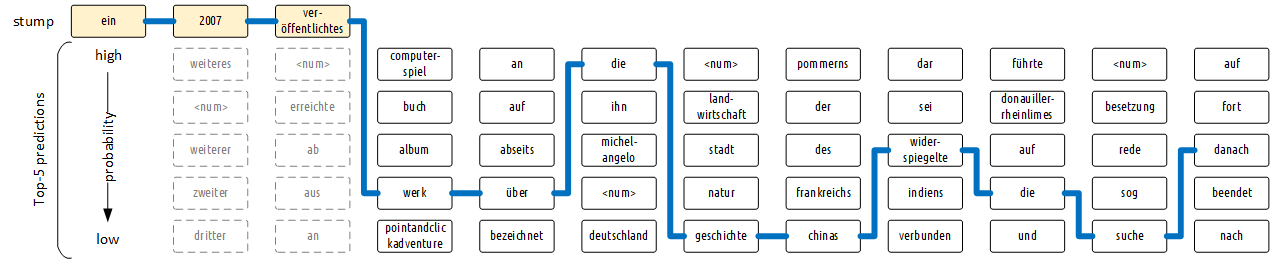
\includegraphics[width=\linewidth]{./img/word_predictor.png}
	\caption{Word predictions of the trained 5-gram model for continuations of the stump \foreignquote*{french}{\textit{Ein 2007 erschienenes ...}}. The blue path represents a grammatically valid German sentence.}
	\label{word_predictor}
\end{figure}

Although prediction was slow we can observe that the words suggested by the \ac{LM} are generally grammatically correct continuations and often make sense, although the probability for some of the predicted words (like \textit{Michelangelo}) is sometimes unexplicably high. Nevertheless it was possible to create a valid German sentence from the stump using only the suggested words. The \ac{LM} even seems to have captured some notion about grammatical concepts like German cases (e.g. that \foreignquote{french}{\textit{die Geschichte Chinas}} is more likely than \foreignquote{french}{\textit{die Geschichte China}}). On the other hand we can observe that the meaningfulness of the suggestions decreases with the progress because some long-distance relationships between words are lost for small values of $n$.

\subsection{\ac{STT} model performance}

The observations made when training the simplified Keras model on German audio data are similar to the ones made when training on English data in that the spell-checker will not help and the CTC validation loss will decrease until epoch 15 and then plateau or increase slightly.

When evaluating the \ac{LER} metric on the test set, the best performance was achieved with a regularized model that was trained on 1.000 minutes of audio, including synthesized samples. The average \ac{LER} value was then $0.4918$, which is even better than the $0.5125$ achieved when training on English samples from the \ac{LS} corpus. This result has to be taken with a pinch of salt though, because the test data in the \ac{RL} corpus is not as extensive as the one from the \ac{LS} corpus and it has also not been extracted with the same diligence. 

The effect of regularisation and/or use of synthesized training data can be visualized. Figure \ref{regularization_synthetisation} shows both measures in isolation and in combination. From the plot on the left it becomes evident that transcripts inferred by a regularized model will generally have a lower \ac{LER} than without regularisation. The plot in the middle shows how the use of synthesized training data has a smoothing effect on the curve of the \ac{LER}. Finally, the plot on the right shows the progress of the average \ac{LER} values when combining both measures, i.e. training a regularized model with training data including synthesized samples. The effect is bot a smoother curve and mostly lower \ac{LER} rates, although there is an awkward spike between epoch 15 and 20.

\begin{figure}[h!]
	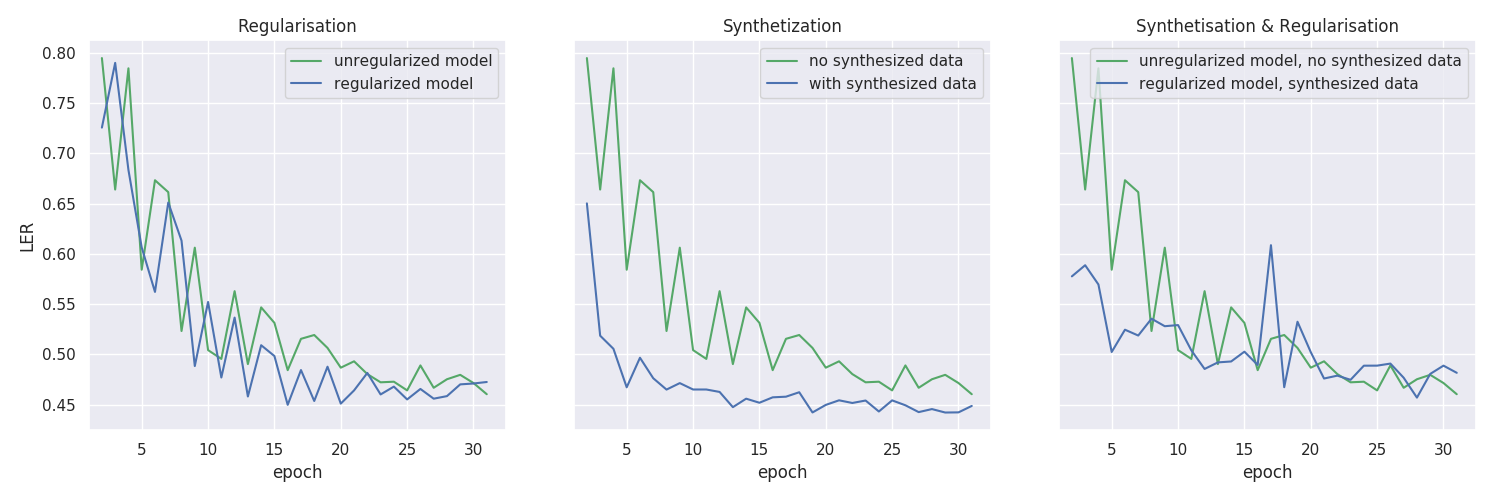
\includegraphics[width=\linewidth]{./img/regularization_synthetisation.png}
	\caption{Impact of regularization and/or synthetisation on the progress of average \ac{LER} values. Regularization alone (left) will lead to lower \ac{LER} rates. Synthesized training data (middle) will lead to a smoother curve and lower \ac{LER} rates. Both measures combined will also combine their effects, although the trend is less obvious.}
	\label{regularization_synthetisation}
\end{figure}

\subsection{Pipeline performance}

Because the regularized model trained with synthesized data has both the lowest \ac{LER} rates and a smoother curve, this model is used in the \ac{ASR} stage of the pipeline when aligning German samples. The pipeline can then be evaluated like it was evaluated for English samples. However, while for English samples the Mozilla implementation of \textit{DeepSpeech} could be used as a reference model, such a reference model is not available for German\footnote{except proprietary \ac{STT} engines like \textit{Google Cloud Speech}, which are only available online} because the \textit{CommonVoice} German dataset is not mature enough. To still evaluate how well the pipeline does for German audio/transcript samples, the segmentation information available in the test data is used instead of splitting the audio signal into voiced parts. The speech segments are put through the other stages (\ac{ASR} and \ac{GSA}) like before. By doing so, the \ac{VAD} stage is canceled out and the results reflect the impact of the last two stages. The final alignments are then evaluated as before, i.e. by calculating $P$recision, $R$ecall and $F$-score, but without comparing the values to a reference model. Because there was no reference model, the inferred transcripts were not concatenated and compared to the original transcript.

\subsection{Summary}

This gave an overview on how $n$-gram \ac{LM} work and how a $5$-gram model for German similar to the one downloaded from Mozilla was trained on Wikipedia corpus and validated empirically. It also showed how a pipeline was built that aligns German audio/text samples. A \ac{STT} model was trained using augmented data from \textit{ReadyLingua}. Like with the English samples, the training progress was visualized with a learning curve. The best performance was achieved using an unregularized model that has been trained on $1.000$ minutes of original and synthetisized data. Likewise the pipeline performance was evaluated, yielding similar results like the English pipeline. However, the pipeline was evaluated on only 6 samples (12 minutes 29 seconds). This is not enough and does not reflect a realistic distribution of speakers, genders, accents, etc. The pipeline for German needs to be evaluated further to make statements about its general capability.